\section{An Algorithm for Relaxed Ring Loading}
\label{sec:relaxed-ring-loading}

We begin by deriving an algorithm for \RRL.

\subsection{Minimal Solutions}

We aim to find a special kind of solution:

\begin{definition}
	Let $\Phi^\ast$ be an optimal solution to an instance of \RRL.
	We say that $\Phi^\ast$ is \emph{minimal} if there exists no other optimal routing $\Phi'$ such that $L_i(\Phi') \leq L_i(\Phi^\ast)$ for all $1 \leq i \leq n$ and $L_j(\Phi') < L_j(\Phi^\ast)$ for at least one $j$.
\end{definition}
While this definition might seem arbitrary at first glance, minimal solutions are of a particularly aesthetic form.

\begin{theorem}
	\label{theo:number-of-splits}
	Let $\Phi^\ast$ be a minimal solution to an instance of \RRL of size $n$.
	Then $\Phi^\ast$ splits at most $\lfloor \frac{n}{2} \rfloor$ demands.
\end{theorem}

This result is quite remarkable, as we can have up to $\binom{n}{2} = \frac{n(n-1)}{2}$ non-zero demands.
This means that a minimal solution to \RRL is already almost binary.
We will later use this fact to obtain a true binary routing which approximates the optimal routing in the corresponding \RL instance.

Before proving the theorem, it is sensible to introduce some additional notation and terminology.
From now on, for the sake of simpler notation, we consider the \RRL instance size $n \in \N$ as fixed.
\begin{notation}
	Let $i, j \in \N$ with $i < j$.
	We define the half-open intervals
	\begin{enumerate}
 		\item $[i, j) \coloneqq \{i, i+1, \ldots, j-1\}$;
 		\item $[j, i) \coloneqq \{j, j+1, \ldots, n-1, n, 1, 2, \ldots, i-1\}$.
	\end{enumerate}
	Open and closed intervals are defined similarly.
\end{notation}
\begin{definition}
	Let $i, j, u, v \in [n]$, $i < j, u < v$ and $d_{i,j}, d_{u, v}$ be two demands of a \RRL instance.
	We say that
	\begin{enumerate}
		\item $d_{i, j}$ and $d_{u, v}$ are \emph{crossing} if $i, j, u, v$ are pairwise distinct and $i < u < j < h$ or $u < i < h < j$.
		\item $d_{i, j}$ and $d_{u, v}$ are \emph{parallel} if they are not crossing.
		\item If $d_{i, j}$ and $d_{u, v}$ are parallel, the edge $\{k, k+1\}$ is \emph{in between}
		$d_{i,j}$ and $d_{u, v}$ if it lies on the front route of exactly one of the demands.
	\end{enumerate}
\end{definition}
Crossing and parallel demands are most easily understood visually.
See \cref{fig:parallel-demands} for some examples.

\begin{figure}
	\centering
	\begin{minipage}[t]{.4\textwidth}
		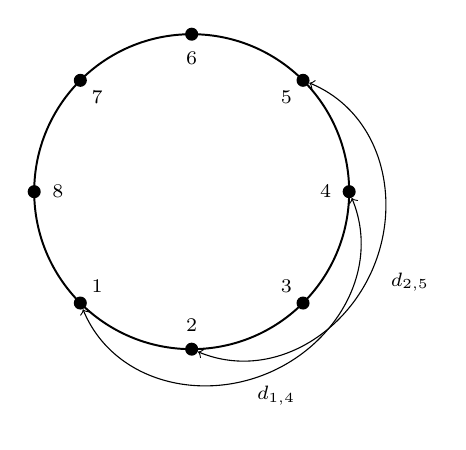
\begin{tikzpicture}[font=\scriptsize, node/.style={circle,thick,draw},
		l_2/.style={line width =0.25mm},
		scale=1, transform shape]
		% equidistant points and arc
		\foreach \x [count=\p] in {0,...,7} {
			\node[shape=circle,fill=black, scale=0.5] (\p) at (\x*45-135:2) {};
		};
		\foreach \x [count=\p] in {0,...,7} {
			\draw (225 + \x*45:1.7) node {\p};
			%				\draw (-30-\x*60:2.4) node {$\bar{\p}$};
		}; 
		\draw[l_2] (4) arc (0:360:2);
		\node (a) at (-22.5:3) {$d_{2, 5}$};
		\draw[<->] (2)  to [out=-22.5,in=-112.5] (-22.5:2.5) to [out=67.5,in=-22.5](5);
		\node (b) at (-67.5:2.8) {$d_{1, 4}$};
		\draw[<->] (1)  to [out=-67.5,in=-157.5] (-67.5:2.5) to [out=22.5,in=-67.5] (4);
		
		\node (bottom) at (0, -2.8) {};
		%		\draw[dashed] (1) -- (3) -- (5) -- (1);
		% axes
		%		\draw [dotted, gray] (-2.6,0) -- (2.6,0);
		%		\draw [dotted, gray] (0,-2.15) -- (0,2.15);
		\end{tikzpicture}
		\subcaption{$d_{1, 4}$ and $d_{2, 5}$ are crossing.}
	\end{minipage}
	%	\hspace{1cm}
	\begin{minipage}[t]{.4\textwidth}
		\begin{tikzpicture}[font=\scriptsize, node/.style={circle,thick,draw},
		l1_green/.style={thick, green!80!black},
		l1_red/.style={thick, blue!80!white},
		l_2/.style={},
		l_3/.style={line width =0.25mm},
		scale=1, transform shape]
		\draw[l_3] (2, 0) arc (0:360:2);
		
		\draw[l1_green] (5) arc (45:90:2);
		\draw[l1_green] (8) arc (180:270:2);
		\draw[l1_red] (4) arc (0:45:2);
		% equidistant points
		\foreach \x [count=\p] in {0,...,7} {
			\node[shape=circle,fill=black, scale=0.5] (\p) at (\x*45-135:2) {};
		};
		% labels
		\foreach \x [count=\p] in {0,...,7} {
			\draw (225 + \x*45:1.7) node {\p};
			%				\draw (-30-\x*60:2.4) node {$\bar{\p}$};
		};
		
		\node (a) at (10:2.9) {$d_{2, 5}$};
		\draw[l_2, <->] (2)  to [out=-22.5,in=-112.5] (-22.5:2.8) to [out=67.5,in=-22.5](5);
		
		\node (b) at (-15:2.46) {$d_{2, 4}$};
		\draw[l_2,<->] (2)  to [out=-15,in=-135] (-45:2.25) to [out=45,in=-75] (4);
		
		\node (c) at (135:2.7) {$d_{6, 8}$};
		\draw[l_2, <->] (6)  to [out=157.5,in=45] (135:2.4) to [out=-135,in=112.5] (8);
		
		\node (bottom) at (0, -2.8) {};
		%		\draw[dashed] (1) -- (3) -- (5) -- (1);
		% axes
		%		\draw [dotted, gray] (-2.6,0) -- (2.6,0);
		%		\draw [dotted, gray] (0,-2.15) -- (0,2.15);
		\end{tikzpicture}
		\subcaption{$d_{2,4}$ and $d_{2, 5}$ and $d_{6, 8}$ are parallel.}
	\end{minipage}
	\caption{Examples of crossing and parallel demands.
		In (b), the green edges lie in between $d_{2, 5}$ and $d_{2, 8}$.
		The blue edge is the only edge in between $d_{2, 4}$ and $d_{2, 5}$.}
	\label{fig:parallel-demands}
\end{figure}

Next, we prove the following lemma.

\begin{lemma}
	\label{lemma:parallel-demands}
	Let $\Phi^\ast$ be a minimal routing and $d_{i, j}$ and $d_{u, v}$ be parallel demands.
	Then no edge in between $d_{i, j}$ and $d_{u, v}$ carries traffic from both demands.
\end{lemma}
\begin{proof}
	Let $\Phi^\ast$ be a minimal solution and assume that the edge $\{k, k+1\}$ lies in between two parallel demands $d_{i, j}, d_{u, v}$ and carries traffic from both demands.
	Let $\alpha$ and $\beta$ be the amounts of traffic from $d_{i,j}$ and $d_{u, v}$, respectively, that are routed through $\{k, k+1\}$.
	Furthermore, assume w.l.o.g. that $\alpha \leq \beta$ and that $\{k, k+1\}$ lies on the front route of $d_{i, j}$ (the other cases can be reasoned analogously).
	
	We now construct a new routing $\Phi'$ from $\Phi^\ast$ by rerouting traffic $\alpha$ of both demands such that it no longer passes through $\{k, k+1\}$.
	This results in $d_{i, j}$ being routed all front or all back.
	The rerouting of $d_{i, j}$ causes the loads on all edges on its front route to decrease by $\alpha$ and those on the back route to increase by $\alpha$.
	Similarly, the rerouting of $d_{u, v}$ increases the loads on all edges on its back route by $\alpha$ and decreases those on its front route by $\alpha$.
	
	Let $\{l, l+1\}$ be any edge.
	Then we can write the load under the new routing as
	\begin{equation}
	L_l(\Phi') = L_l(\Phi^\ast) 
	+ \alpha (\dOne_{\{l \notin [i, j)\}} - \dOne_{\{l \in [i, j)\}} +  \dOne_{\{l \in [g, h)\}} - \dOne_{\{l \notin [g, h)\}} )
	\end{equation}
	Here, $\dOne_{\{\ldots\}}$ is the indicator function that is $1$ if the condition in the index is true and $0$ else.
	We assumed that $\{k, k+1\}$ lies on the front route of $d_{i, j}$, but also that it lies in between $d_{i, j}$ and $d_{g, h}$.
	This implies that $[g, h] \subset [i, j]$.
	Hence $l \notin [i, j)$ and $l \in [g, h)$ cannot both be true at the same time.
	This shows that $L_l(\Phi') \leq L_l(\Phi^\ast)$.
	Furthermore, $k \in [i, j)$ and $k \notin [g, h)$ by definition of $k$.
	Thus we have $L_k(\Phi') < L_k(\Phi^\ast)$.
	Altogether, the existence of the routing $\Phi'$ contradicts the minimality of $\Phi^\ast$.
\end{proof}

With these preparations, we can now conduct the proof of \cref{theo:number-of-splits}.
\begin{proof}[Proof of \cref{theo:number-of-splits}]
	Let $\Phi^\ast$ be a minimal routing and let $S \coloneqq \{(i, j)\ |\ 0 < \Phi^\ast(i, j) < 1\}$ be the set of indices of demands that are split by $\Phi^\ast$.
	Furthermore, let $(i, j), (u, v) \in S$.
	
	If the demands $d_{i,j}$ and $d_{u, v}$ were parallel, there would be a link $\{k, k+1\}$ that carries traffic from both demands, as they are both split.
	However, it follows from the minimality of $\Phi^\ast$ and \cref{lemma:parallel-demands} that this cannot be the case, which implies that $d_{i,j}$ and $d_{u, v}$ are crossing.
	This requires, by definition, that $i, j, u, v$ are mutually distinct.
	
	This implies that every element of $[n]$ can occur in at most one tuple in $S$.
	As the tuples in $S$ each consist of two elements, there can be at most $\lfloor\frac{n}{2}\rfloor$ such tuples.
\end{proof}

The existence of minimal solutions is not clear, a priori.
In the following, we will show that minimal solutions always exist by providing an algorithm.

\subsection{Constructing a Minimal Solution}

In order to construct a minimal solution, we first consider a generalization of \RRL by appending edge capacities $C_k \in \R_{\geq 0}$ for each edge $\{k, k+1\}$.
The resulting problem, \textsc{RelaxedRingLoadingWithCapacities (RRLWC)}, is to determine a real-valued routing $\Phi^\ast$ such that $L_k(\Phi^\ast) \leq C_k$ for all $k \in [n]$.
This problem does not always have feasible solutions.
In the following, we show a necessary and sufficient condition for the existence of feasible solutions.

\begin{definition}
	A \emph{cut} is a set of two distinct edges.
	For $g, h \in [n], g \neq h$, we denote the cut by $\{g, h\}$ instead of $\{\{g, g+1\}, \{h, h+1\}\}$.
\end{definition}

We can imagine a cut $\{g, h\}$ as a chord connecting the edges $\{g, g+1\}$ with the link $\{h, h+1\}$.
A cut therefore "splits" the ring into two parts.

\begin{definition}
	Let $d_{i, j}$ be a demand.
	We say that $d_{i, j}$ \emph{crosses} the cut $\{g, h\}$, if the endpoints of $d_{i, j}$ are on both sides of the cut.
	Formally, this is the case if and only if $\abs{[i, j) \cap (g, h]} = 1$.
\end{definition}

This visualization 
A cut therefore splits the ring into two connected components and can therefore also use the same terms to describe their properties as for demands, such as \emph{crossing} and \emph{parallel}.

\begin{definition}
	The \emph{demand across the cut} $\{g, h\}$ with $g \neq h$ is the sum of demands with endpoints on both sides of the cut:
	\begin{equation}
		\label{eq:cut-demand-definition}
		D_{gh} \coloneqq \sum_{d_{ij} \in \{d_{ij}\ |\ \abs{[i, j) \cap (g, h]} = 1\}} \ .
	\end{equation}
	For the degenerate cuts $\{g, g\}$ we define $D_{gg} \coloneqq 2 C_g$.
\end{definition}

\begin{definition}[Cut Condition]
	An cut $\{g, h\}$ is said to satisfy the \emph{cut condition} if
	\begin{equation}
		D_{gh} \leq C_g + C_h \ .
	\end{equation}
	An instance $I$ \emph{satisfies the cut condition} if each cut does.
	$C_g + C_h - D_{gh}$ is called the \emph{slack} of the cut $\{g, h\}$.
\end{definition}
In an instance of \RRL, is there is a cut $\{g, h\}$ which violates the cut condition, the instance is not solvable:
The links $\{g, g+1\}$ and $\{h, h+1\}$ pose a bottleneck to the demands that cross the cut and hinder every demand from being satisfied.

\begin{theorem}
	\label{theo:cut-condition}
	Let $I$ be an instance of \RRL that satisfies the cut condition.
	Then $I$ is solvable.
\end{theorem}
For the proof, we will need the following lemma:
\begin{lemma}
	\label{lemma:parallel-diagonal-cuts}
	Let $\{g, h\}$, $\{g', h'\}$ be two parallel cuts.
	Then every demand crosses as many of the cuts $\{g, h\}$, $\{g', h'\}$ as it crosses cuts $\{g, g'\}, \{h, h'\}$
\end{lemma}
\begin{proof}
	By distinction of cases.
\end{proof}
\begin{proof}[Proof of \cref{theo:cut-condition}]
	We conduct the proof by assuming there are instances that satisfy the cut condition, but are not solvable.
	Let $I$ be the smallest of these instances in terms of ring size $n$ and the number of non-zero demands.
	
	We now construct another non-solvable instance $I'$ with one less non-zero demand and show that this instance still satisfies the cut condition.
	This will contradict the minimality of $I$, implying that no such instance exists.
	
 	We begin by picking any non-zero demand $d_{ij}$ with $j - i \geq 2$.
	
	If none exists, all non-zero demands in $I$ must be of the form $d_{i, i+1}$.
%	Then neither of these demands can be routed through the front route, that is the link $\{i, i+1\}$, as otherwise we could construct an instance with one less non-zero demand by pretending to route that demand through the front and decreasing the capacity of the link $\{i, i+1\}$ accordingly.
%	This would contradict the minimality of $I$.
%	Hence, the only possibility is to route all demands through the back route, let $\phi$ be that routing.
%	Doing this, for all $1 \leq k \leq n$ the link loads are given as
%	\begin{equation}
%		% All is routed through the back
%		L_k = \sum_{\{d_{ij}\ |\ k \notin [i, j)\}} d_{ij} \leq D_{kl} \leq C_k + C_l \quad \forall l\neq k \ .
%	\end{equation}
%	This means that $\phi$ solves $I$, contradicting the non-feasibility of $I$. 
	Pick any such demand $d_{i, i+1}$ of which there must be at least one, as otherwise any routing solves $I$.
	Then, renumber the nodes and links by "rotating" such that $d_{i, i+1}$ corresponds to $d_{1, n}$ in the renumbered instance, which still satisfies minimality in the above sense.
	Continue with the new instance in which it is possible to pick a non-zero demand $d_{ij}$ with $j - i \geq 2$, as $n \geq 4$.
	
	Hence, we have a non-zero demand with $j - i \geq 2$. 
	Let $\{g, h\}$ be a cut with minimal slack $M$ along the front route of $d_{ij}$, that is a cut $\{g, h\}$ with $i \leq g < h < j$ that minimizes $C_g + C_h - D_{gh}$.
	We construct a new instance $I'$ by pretending to route $\frac{M}{2}$ traffic of $d_{ij}$ along the front route and the remaining $d_{ij} - \frac{M}{2}$ along the back route.
	We set the capacities of the new instance accordingly, that is $C_k' = C_k - \frac{M}{2}$ for links on the front route and $C_k' = C_k - (d_{ij} - \frac{M}{2})$ on the back route.
	The demands remain the same with the exception of $d_{ij}$, which is now $0$.
	It is easy to see that the new instance is still not solvable; otherwise we could use any feasible routing for $I'$ to construct a solution to $I$.
	
	By construction, all cuts $\{s, t\}$ in $I'$ that lie on the front route of $d_{ij}$, that is $i \leq s < t < j$, still satisfy the cut condition:
	\begin{equation}
		D_{st}' = D_{st} \leq C_{s} + C_{t} - M = (C_{s} - \frac{M}{2}) + (C_{t} - \frac{M}{2}) \stackrel{\mathrm{Def.}}{=} C_{s}' + C_{t}' \ .
	\end{equation}
	The first equality follows from the fact that $d_{ij}$ does not contribute to $D_{st}$ and $D_{st}'$, the inequality from the choice of $M$.
	Similarly, all cuts $\{s, t\}$ that $d_{ij}$ crosses satisfy the cut condition.
	Assume $s \notin [i, j), t \in [i, j)$ without loss of generality, then the following holds true:
	\begin{equation}
		D_{st}' = D_{st} - d_{ij} \leq C_s + C_t - d_{ij} = \left(C_s - \left(d_{ij} - \frac{M}{2}\right)\right) + \left(C_h - \left(d_{ij} - \frac{M}{2}\right)\right) \stackrel{\mathrm{Def.}}{=} C_s' + C_t' \ .
	\end{equation}
	Here, the first equality results from $d_{ij}$ no longer contributing to the demand of cuts which it crosses.
	The inequality is simply the cut condition in $I$.
	
	Now, pick any cut $\{s, t\}$ which lies on the back route of $d_{ij}$ and assume it violates the cut condition.
	This means that
	\begin{equation}
		D_{st} = D_{st}' > C_s' + C_h' \stackrel{\mathrm{Def.}}{=} \left(C_s - \left(d_{ij} - \frac{M}{2}\right)\right) + \left(C_h - \left(d_{ij} - \frac{M}{2}\right)\right)
	\end{equation}
	or equivalently $D_{st} +  2(d_{ij} - \frac{M}{2}) > C_s + C_h$.
	This, the choice of $M$ and \cref{lemma:parallel-diagonal-cuts} implies that
	\begin{align}
		D_{sg} + D_{th} &\geq D_{gh} + D_{st} + 2 d_{ij}\\
		&> (C_g + C_h - M) +  \left(C_s - \left(d_{ij} - \frac{M}{2}\right)\right) + \left(C_h - \left(d_{ij} - \frac{M}{2}\right)\right) + 2 d_{ij}\\
		&= C_g + C_h + C_s + C_t \ .
	\end{align}
%	In the inequality we further used the fact that $D_{gh} = C_g + C_h - M$.
	In total, this means that $D_{sg} > C_s + C_g$ or $D_{th} > C_t + C_h$, showing that at least one of the cuts $\{s, g\}$, $\{t, h\}$ has violated the cut condition in $I$; a contradiction.
	
	Thus all cuts in the new instance $I'$ satisfy the cut condition.
	This contradicts the minimality of $I$ which shows that no such instance can exist.
\end{proof}

As we have seen, \RRL can be formulated as a linear program and thus be solved as such.
This can be done e.g. using XXYYs algorithm, which requires $\cO(??)$ time in our application.
There is, however, another method which is significantly faster.
The method is described in \cref{algo:rrl}


\begin{figure}[ht]
	\begin{algorithm}[H]
		\KwData{Ring size $n \in \N$, demands $d_{ij}$, $1 \leq i < j \leq n$.}
		$M = \max_{1 \leq i < j \leq n} D_{ij}$\;
		\For{$i=1, \ldots, n$}{
			$C_i = \max \left(\max_{1 \leq j < i}(D_{ji} - C_j), \max_{i < j \leq n}(D_{ij} - \frac{M}{2})\right)$ \;
		}
		\While{$\exists \text{parallel demands } d_{ij}, d_{gh}$}{
			Choose link $\{k, k+1\}$ that lies in between $d_{ij}$ and $d_{gh}$\;
			$\{k, l\} \coloneqq \min_{l \neq k} C_k + C_l - D_{kl}$\;
			Assume $d_{ij}$ crosses $\{k, l\}$\;
			Route $d_{gh}$ such that it misses $\{k, l\}$\;
			// Wollen cut constraint als Invariante idealerweise
		}
%		\While{not converged}{
%			\For{$i=1, \ldots, k$}{
%				Sample batch of $B$ samples $z_1, \ldots, z_B$ from $p_z$\;
%				Sample batch $x_{i_1}, \ldots, x_{i_B}$ from the training data\;
%				Compute the stochastic gradient 
%				$$\nabla_{\theta_D} \frac{1}{B} \sum_{j=1}^{B} \left( \ln D(x_{i_j}) + \ln(1 - D(G(z_j))) \right);$$
%				Update $\theta_D$ by ascending the gradient according to the learning rule $R$\;
%			}
%			Sample batch of $B$ samples $z_1, \ldots, z_B$ from $p_z$\;
%			Compute the stochastic gradient
%			$$\nabla_{\theta_G} \frac{1}{B} \sum_{j=1}^{B} -\ln(D(G(z_j)));$$
%			Update $\theta_G$ by descending the gradient according to the learning rule $R$\;
%		}
		\Return{$\phi$}
		\caption{Algorithm for \RRL}
		\label{algo:rrl}
	\end{algorithm}
\end{figure}

\input{figures/demand_cuts_algorithm}

\begin{align}
	M &\coloneqq \max_{1 \leq i < j \leq n} D_{ij}\\
	\label{eq:minimal-capacities}
	C_i &\coloneqq \max \left(\max_{1 \leq j < i}(D_{ji} - C_j), \max_{i < j \leq n}(D_{ij} - \frac{M}{2})\right)
\end{align}

\begin{lemma}
	\label{lemma:capacities-bounded}
	Let $I$ be an instance of \RRL and let the capacities $C_i$ be defined as in \cref{eq:minimal-capacities}.
	Then $C_i \leq \frac{M}{2}$ for all $1 \leq i \leq n$.
\end{lemma}
\begin{proof}
	We conduct the proof by induction over $i$. 
	The beginning $i=1$ is covered in Case 2 below. 
	Thus, Let $2 \leq i \leq n$.
	We distinguish two cases:
	\begin{enumerate}[align=left]
		\item[Case 1: $C_i = \max_{1 \leq j < i}(D_{ji} - C_j)$]{\mbox{}\\
			Then there exists some $1 \leq j < i$ for which we have
			\begin{align}
				C_i &= D_{ji} - C_j \\
				&\stackrel{\mathrm{IH}}{\leq} D_{ji} - \left(\max_{j < k \leq n} D_{jk} - \frac{M}{2}\right)\\
				&= (D_{ji} - \max_{j < k \leq n} D_{jk}) + \frac{M}{2} \ .
			\end{align}
			Because of $j < i$ we have $D_{ji} - \max_{j < k \leq n} D_{jk} \leq 0$, proving that $C_i \leq \frac{M}{2}$.
		}
		\item[Case 2: $C_i = \max_{i < j \leq n}(D_{ij} - \frac{M}{2})$]{\mbox{}\\
			Then it immediately follows from the choice of $M$ that $C_i \leq M - \frac{M}{2} = \frac{M}{2}$.
		}
	\end{enumerate}
\end{proof}

\begin{lemma}
	\label{lemma:minimal-solution}
	Let $I$ be an instance of \RRL.
	Let $M \coloneqq \max_{1 \leq i < j \leq n} D_{ij}$ and let $C_i$ be such as to satisfy $C_i = \max \left(\max_{1 \leq j < i}(D_{ji} - C_j), \max_{i < j \leq n}(D_{ij} - \frac{M}{2})\right)$ for all $1 \leq i \leq n$.
	Then any routing $\phi$ for $I$ which does not violate the capacities $C_i$ is minimal with ring load $L = \frac{M}{2}$.
\end{lemma}
\begin{proof}
	Let $\{g, h\}$ be the cut for which the maximum $M$ is attained.
	Then in any feasible routing, at least $\frac{M}{2}$ traffic must be routed through either of the links $\{g, g+1\}$, $\{h, h+1\}$, implying that $L \geq \frac{M}{2}$.
	However, the instance $I$ together with the capacities $C_i = \frac{M}{2}$ for all $1 \leq i \leq n$ satisfies the cut constraint.
	It follows from \cref{theo:cut-condition} that a solution exists, which by construction has a ring load $L \leq \frac{M}{2}$.
	Together we get $L = \frac{M}{2}$.
	
	The capacities $C_i$ are such that $I$ satisfies the cut condition:
	For $1 \leq i < j \leq n$ we have
	\begin{equation}
		C_j = \max \left(\max_{1 \leq k < j}(D_{kj} - C_k), \max_{j < k \leq n}(D_{jk} - \frac{M}{2})\right) \geq D_{ij} - C_i \ ,
	\end{equation}
	which implies $D_{ij} \leq C_i + C_j$.
	Thence by \cref{theo:cut-condition} there exists a solution to $I$ which does not violate the link capacities.
	Let $\phi$ such a routing with link loads $L_i$.
	We now show that $\phi$ is minimal by contraposition.
	
	Therefore, assume that $\phi$ is not minimal and let $\phi'$ with link loads $L_i'$ be a witness.
	We define new capacities $C_i' \coloneqq L_i'$ for all $1 \leq i \leq n$.
	Especially, we have $C_i' \leq C_i$ for all $i$ and $C_k' < C_k$ for at least one $k$.
	Let $j$ be the smallest index for which $C_j' < C_j$.
	We now show that there is a cut $\{j, l\}$ which violates the cut condition for the capacities $C_i'$ by distinguishing the two possible cases:
	\begin{enumerate}[align=left]
		\item[Case 1: $C_j = \max_{1 \leq k < j}(D_{kj} - C_k)$]{\mbox{}\\
			The we especially have $C_j' < C_j = \max_{1 \leq k < j}(D_{kj} - C_k)$ and by the choice of $j$ as the smallest index $C_i' = C_i$ for all $1 \leq i < j$.
			This means that there exists a $1 \leq k \leq j$ such that $C_j' < D_{kj} - C_k = C_j' < D_{kj} - C_k'$, implying that $D_{kj} > C_k' + C_j'$.
			Thus, the cut $\{k, j\}$ is violated.
		}
		\item[Case 2: $C_j = \max_{j < k \leq n}(D_{jk} - \frac{M}{2})$]{\mbox{}\\
			Then $C_j' < C_j = \max_{j < k \leq n}(D_{jk} - \frac{M}{2})$.
			This means that there exists a $j < k \leq n$ such that $C_j' < D_{jk} - \frac{M}{2}$.
			Using \cref{lemma:capacities-bounded} we then get 
			\begin{equation}
				C_j' + C_k' \leq C_j' + C_k \leq C_j' + \frac{M}{2} < D_{jk} \ ,
			\end{equation}
			again showing that the cut $\{k, j\}$ is violated.
		}
	\end{enumerate}
	In total this shows that the instance $I'$ with capacities $C_i'$ does not satisfy the cut condition.
	Thus there exists no witness $\phi'$, proving that $\phi$ already was minimal.
\end{proof}

The following theorem guarantees that the algorithm works correctly.
\begin{theorem}
	\label{theo:rll-algo-correct}
	Let $I$ be an instance of size $n$ of \RRL that satisfies the cut condition.
	Then \cref{algo:rrl} computes a minimal solution of $I$ in $\cO(n^2)$ time using $\cO(?)$ space.
\end{theorem}
\begin{proof}
	Computing the $\binom{n}{2}$ values $D_{ij}$ can be done in $\cO(n^4)$ time in the obvious way, using the formula in \cref{eq:cut-demand-definition}.
	However, there exists a more efficient way which is described in \cref{algo:demands-across-cuts}.
	This improved algorithm completes the task in $\cO(n^2)$, which is optimal (it already takes $\Omega(n^2)$ time to read the $\binom{n}{2}$ inputs $d_{ij}$).
	This subroutine is based on the following recursion:
	\Todo{Maybe add proper proof if there is space, otherwise explain basic idea in one sentence.}
	\begin{equation}
		D_{i, j} = \begin{cases}
			\sum_{k < i+1} d_{k,i+1} + \sum_{k > i+1} d_{i+1, k}, & \text{if } j = i+1 \\
			D_{i, i+1} + D_{i+1, j} - 2 A_{i+1, j}, & \text{if } j > i+1
		\end{cases}
	\end{equation}
	where we used the auxiliary variables $A_{i, j}$ that are defined as follows:
	\begin{equation}
		A_{i, j} \coloneqq \begin{cases}
				d_{i, i+1}, & \text{if } j = i+1\\
				A_{i, j-1} + d_{i, j}, &\text{if } j > i+1\\
		\end{cases}
	\end{equation}
	Applying the maximum operator to the $\binom{n}{2}$ values $D_{ij}$ also takes $\cO(n^2)$ time.
	
	The computation of the capacities $C_i$ can be carried out in $\cO(n^2)$ time:
	Each iteration of the for-loop takes time linear in $n$, as the maximum of at most $n$ values is taken.
	
	For the correctness we just have to understand that the algorithm does indeed compute a solution $\phi$ which does not violate the capacities $C_i$.
	\cref{lemma:minimal-solution} then guarantees the minimality of the solution.
	
	
\end{proof}

\begin{lemma}
	For all $i \in [n]$ let $L_i^f$ and $L_i^b$ be the total traffic that is routed forward and backward, respectively, through the link $\{i, i+1\}$.
	Then for any routing $\phi$, the following recursions hold true.
	\begin{align}
		L_i^f &\coloneqq \begin{cases}
			\sum_{j = 2}^n d_{1j} \cdot \phi(1, j), & \text{if } i = 1 \\
			L_{i-1}^f - \sum_{j = 1}^{i-1} d_{ji} \cdot \phi(j, i) + \sum_{j = i}^{n} d_{ij} \cdot \phi(i, j) & \text{if } i > 1 \\
		\end{cases} \\
		L_i^b &\coloneqq \begin{cases}
		\sum_{i = 1}^n \sum_{j = i+1}^n d_{ij} \cdot (1 - \phi(i, j)) & \text{if } i = n\\
		L_{(i-1)\mod n} - \sum_{j = i}^{n} d_{i, j} \cdot (1 - \phi(i, j)) + \sum_{j = 1}^{i-1} d_{ij} \cdot(1 - \phi(i, j)) & \text{if } i < n
		\end{cases} \ 
	\end{align}
\end{lemma}

\begin{lemma}
	At the beginning of the while-loop in \cref{algo:rrl}, for every $i \in [n]$ there exists a $j \neq i$ such that $\{i, j\}$ is a tight cut.
\end{lemma}
\begin{proof}
	Assume the contrary, that is there is an $i \in [n]$ which is not part of any tight cut.
	Let $M \coloneqq \min_{j \neq i} C_i + C_j - D_{ij}$.
	Then $M > 0$ by assumption.
	Define $C_i' = C_i - M$ and $C_j' = C_j$ for all $j \neq i$.
	Then every cut still satisfies the cut condition.
	But in the proof of \cref{lemma:minimal-solution} we showed that no such set of capacities can exist.
\end{proof}

\begin{theorem}
	Let $T$ be the set of tight cuts at the beginning of \cref{algo:rrl} and let $Q$ be the set of demands that cross all cuts in $T$.
	Then:
	\begin{itemize}
		\item all demands in $Q$ are mutually crossing.
		\item $\abs{Q} \leq n$ (probably even $\abs{Q} \leq \frac{n}{2}$)
		\item Let $m$ be the minimal number of cuts such that there exists a set $M$ with $m = \abs{M}$ and every demand crosses at least one cut in $M$. Then $\abs{T} \geq m$.
	\end{itemize}
\end{theorem}

\begin{lemma}
	Once a cut becomes tight in \cref{algo:rrl}, it remains tight.
\end{lemma}
\begin{proof}
	There are two points in \cref{algo:rrl} where the slack of a cut can change:
	When the capacities are decreased and when the $D_{ij}$ change.
	First, note that decreasing the capacities can only decrease slack.
	This cannot un-tighten any cut.
	Second, when any $D_{ij}$ changes it must be due to a crossing demand $d_{gh}$ being routed either way.
	This means that the new demand across the cut is $D_{ij}' = D_{ij} - d_{gh}$.
	However, in this case the capacity of either $\{i, i+1\}$ or $\{j, j+1\}$ is also decreased by $d_{gh}$, meaning that
	$C_i' + C_j' = C_i + C_j - d_{gh}$.
	In total we get $C_i' + C_j' - D_{ij}' = C_i + C_j - D_{ij}$, showing that the slack does not change.
\end{proof}

\begin{lemma}
	Let $\{u, v\}$ be a tight cut and $d_{ij}$ be a demand parallel to $\{u, v\}$.
	Then in any solution, $d_{ij}$ must be routed to miss the cut.
\end{lemma}
\begin{proof}
	In any solution, all demands that cross the cut $\{u, v\}$ must route their traffic through $\{u, u+1\}$ or $\{v, v+1\}$ (or both).
	The sum of all such demands is just $D_{uv} = C_u + C_v$, which means that these demands already saturate both links $\{u, u+1\}$ and $\{v, v+1\}$.
	This implies that no demand that does not cross the cut can be routed through those links. 
\end{proof}

\begin{lemma}
	\label{lemma:number-of-split-demands}
	At the end of \cref{algo:rrl} at most $\lfloor\frac{n}{2}\rfloor$ demands are split.
\end{lemma}
\begin{proof}
	Let $\phi^\ast$ be the minimal routing that results from the execution of \cref{algo:rrl}.
	Furthermore, let $S \coloneqq \{(i, j)\ |\ d_{ij}\ \text{is split by}\ \phi^\ast \}$ and $(i, j), (g, h) \in S$.
	If the demands $d_{ij}$ and $d_{gh}$ were parallel, there would be a link $\{k, k+1\}$ that carries traffic from both demands, as they are both split.
	However, it follows from the minimality of $\phi^\ast$ and \cref{theo:parallel-demands-non-crossing} that this cannot be the case, which implies that $d_{ij}$ and $d_{gh}$ are crossing.
	This can, by definition, only occur if $i, j, g, h$ are mutually distinct.
	
	This implies that every $1 \leq i \leq n$ can occur in at most one tuple in $S$.
	As the tuples in $S$ each consist of two elements, there can be at most $\lfloor\frac{n}{2}\rfloor$ such tuples.
\end{proof}

\subsection{Correctness}

\subsection{Runtime}


\begin{proof}
\end{proof}